\documentclass[11pt]{article}

\usepackage[margin=1in]{geometry}
\usepackage{amsmath, amssymb}
\usepackage{booktabs}
\usepackage{hyperref}
\usepackage{braket}
\usepackage{pgfplots}
\pgfplotsset{compat=1.18}

\title{CSE 4412: Introduction to Quantum Computing \\ Homework 1 --- Chapter 2 Exercises}
\author{}
\date{}

\begin{document}
\maketitle

\section*{Exercise 2.2}
\textbf{Statement.} Let $\ket{+} = \frac{1}{\sqrt{2}}(\ket{0} + \ket{1})$ and $\ket{-} = \frac{1}{\sqrt{2}}(\ket{0} - \ket{1})$. Compute $\braket{+|+}$, $\braket{+|-}$, and $\braket{-|-}$. What can you say about these two vectors? You may use the fact that $\ket{0}$ and $\ket{1}$ are orthonormal.

\textbf{Solution.} Using bilinearity of the inner product and $\braket{0|0} = \braket{1|1} = 1$, $\braket{0|1} = \braket{1|0} = 0$:
\begin{align*}
\braket{+|+} &= \frac{1}{2}\left(\braket{0|0} + \braket{0|1} + \braket{1|0} + \braket{1|1}\right) = \frac{1}{2}(1 + 0 + 0 + 1) = 1, \\
\braket{+|-} &= \frac{1}{2}\left(\braket{0|0} - \braket{0|1} + \braket{1|0} - \braket{1|1}\right) = \frac{1}{2}(1 - 0 + 0 - 1) = 0, \\
\braket{-|-} &= \frac{1}{2}\left(\braket{0|0} - \braket{0|1} - \braket{1|0} + \braket{1|1}\right) = \frac{1}{2}(1 - 0 - 0 + 1) = 1.
\end{align*}
Since $\braket{+|+} = \braket{-|-} = 1$, both $\ket{+}$ and $\ket{-}$ are normalized. Since $\braket{+|-} = 0$, they are orthogonal to each other. Therefore $\{\ket{+}, \ket{-}\}$ is an orthonormal set, and since it consists of two linearly independent vectors in the 2-dimensional space $\mathbb{C}^2$, it forms an orthonormal basis (the Hadamard basis).

\section*{Exercise 2.4}
\textbf{Statement.} Consider the following three questions:
\begin{enumerate}
    \item Consider the $\ket{+}$ state. What is the probability of observing $\ket{1}$ after a measurement?
    \item Consider $\ket{-} = \frac{1}{\sqrt{2}}(\ket{0} - \ket{1})$. What is the probability of observing $\ket{1}$ after measuring that state?
    \item Consider the state $\ket{1}$. What is the probability of observing $\ket{1}$ after measurement?
\end{enumerate}

\textbf{Solution.} Recall that for a state $\ket{\psi} = \alpha\ket{0} + \beta\ket{1}$, the probability of observing outcome $\ket{1}$ is $|\beta|^2$.
\begin{enumerate}
    \item For $\ket{+} = \frac{1}{\sqrt{2}}\ket{0} + \frac{1}{\sqrt{2}}\ket{1}$, the coefficient of $\ket{1}$ is $\beta = \frac{1}{\sqrt{2}}$, so
    \[
    \Pr(\ket{1}) = \left|\frac{1}{\sqrt{2}}\right|^2 = \frac{1}{2}.
    \]
    \item For $\ket{-} = \frac{1}{\sqrt{2}}\ket{0} - \frac{1}{\sqrt{2}}\ket{1}$, the coefficient of $\ket{1}$ is $\beta = -\frac{1}{\sqrt{2}}$, so
    \[
    \Pr(\ket{1}) = \left|-\frac{1}{\sqrt{2}}\right|^2 = \frac{1}{2}.
    \]
    \item For $\ket{1}$ itself, $\alpha = 0$ and $\beta = 1$, so
    \[
    \Pr(\ket{1}) = |1|^2 = 1.
    \]
\end{enumerate}

\section*{Exercise 2.5}
\textbf{Statement.} Imagine you are given a qubit $\ket{\psi}$ but not told anything about it (i.e., you do not know its probability amplitudes). If you perform a measurement on the state and the outcome is ``0,'' what does this tell you about the state? Can you learn the original probability amplitudes? What if you are given as many copies of $\ket{\psi}$ as you want -- what can be said then?

\textbf{Solution.} Write $\ket{\psi} = \alpha\ket{0} + \beta\ket{1}$ with $|\alpha|^2 + |\beta|^2 = 1$.

A single measurement that yields outcome ``0'' tells you two things: (1) that $\alpha \neq 0$ (otherwise outcome ``0'' would have occurred with probability zero), and (2) that, due to state collapse, the state \emph{after} the measurement is now exactly $\ket{0}$, regardless of what $\alpha$ and $\beta$ originally were. It does \emph{not} let you recover the original amplitudes $\alpha, \beta$: measurement is an inherently random, information-destroying process, and a single classical outcome (one bit) cannot be inverted to reveal two continuous complex parameters. Many different states (any $\alpha \neq 0$) could have produced this same outcome, each with different probability, so a single trial is consistent with infinitely many possible original states.

If you are given many independently prepared copies of $\ket{\psi}$ (note: this must mean you are handed additional copies from the source, since the no-cloning theorem forbids copying an \emph{unknown} qubit yourself), you can measure each copy in the computational basis and record the fraction of ``0'' and ``1'' outcomes. By the law of large numbers, as the number of copies $n \to \infty$, the empirical frequency of ``0'' converges to $|\alpha|^2$ (and similarly the frequency of ``1'' converges to $|\beta|^2$). So you can learn $|\alpha|^2$ and $|\beta|^2$ to arbitrary precision. However, even with infinitely many copies, measuring only in a single fixed basis can never reveal the relative phase between $\alpha$ and $\beta$ (equivalently, only the magnitudes are learned, not the full complex amplitudes) -- to estimate that you would additionally need to measure copies in other bases (e.g., the Hadamard basis) and combine the statistics.

\section*{Exercise 2.6}
\textbf{Statement.} Let $p \in [0,1]$ be a real number and consider the state
\[
\ket{\psi} = \sqrt{p}\,\ket{0} + \sqrt{1-p}\,\ket{1}.
\]
Answer the following: (1) probability of observing $\ket{0}$ for a given $p$; (2) probability of observing $\ket{-}$ for a given $p$; (3)--(4) graph both probability distributions as functions of $p$.

\textbf{Solution.}

\textbf{(1)} The coefficient of $\ket{0}$ is $\sqrt{p}$, so
\[
\Pr(\ket{0}) = |\sqrt{p}|^2 = p.
\]

\textbf{(2)} Using the inner-product rule, $\Pr(\ket{-}) = |\braket{-|\psi}|^2$:
\begin{align*}
\braket{-|\psi} &= \frac{1}{\sqrt{2}}\left(\braket{0} - \braket{1}\right)\!\cdot\!\left(\sqrt{p}\ket{0} + \sqrt{1-p}\ket{1}\right) = \frac{1}{\sqrt{2}}\left(\sqrt{p} - \sqrt{1-p}\right), \\
\Pr(\ket{-}) &= \left|\frac{\sqrt{p} - \sqrt{1-p}}{\sqrt{2}}\right|^2 = \frac{1}{2}\left(p + (1-p) - 2\sqrt{p(1-p)}\right) = \frac{1}{2} - \sqrt{p(1-p)}.
\end{align*}

\textbf{(3)} Graph of $\Pr(\ket{0}) = p$ versus $p$:
\begin{center}
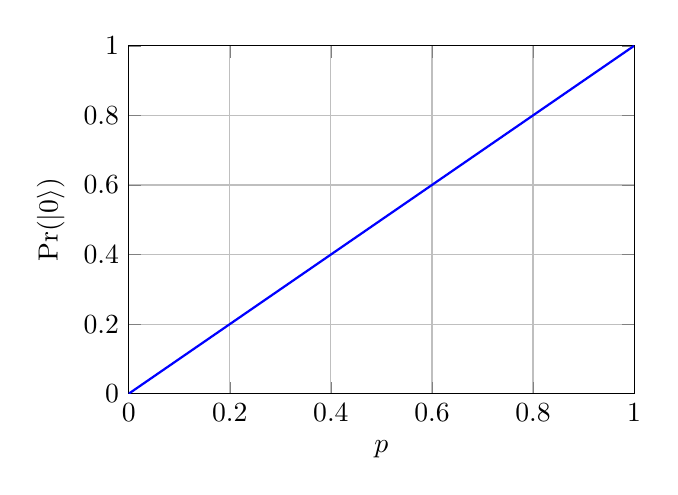
\begin{tikzpicture}
\begin{axis}[
    width=8cm, height=6cm,
    xlabel=$p$, ylabel=$\Pr(\ket{0})$,
    xmin=0, xmax=1, ymin=0, ymax=1,
    domain=0:1, samples=100,
    grid=major
]
\addplot[thick, blue] {x};
\end{axis}
\end{tikzpicture}
\end{center}

\textbf{(4)} Graph of $\Pr(\ket{-}) = \tfrac{1}{2} - \sqrt{p(1-p)}$ versus $p$:
\begin{center}
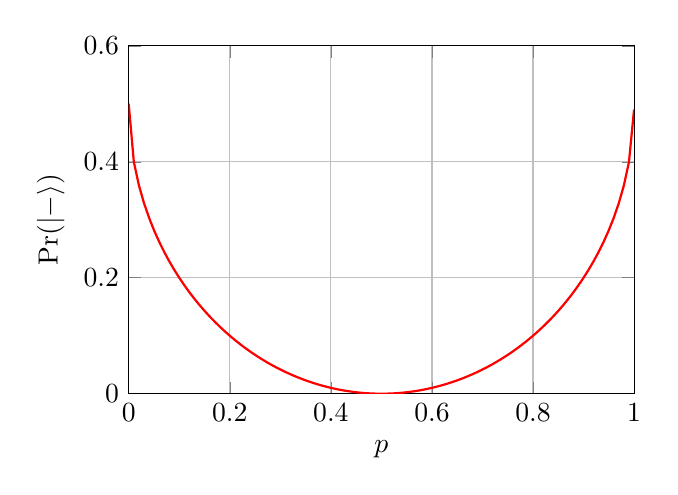
\begin{tikzpicture}
\begin{axis}[
    width=8cm, height=6cm,
    xlabel=$p$, ylabel=$\Pr(\ket{-})$,
    xmin=0, xmax=1, ymin=0, ymax=0.6,
    domain=0:1, samples=100,
    grid=major
]
\addplot[thick, red] {0.5 - sqrt(x*(1-x))};
\end{axis}
\end{tikzpicture}
\end{center}
Note that $\Pr(\ket{-})$ is symmetric about $p = 1/2$, is zero exactly at $p = 1/2$ (where $\ket{\psi} = \ket{+}$, which is orthogonal to $\ket{-}$), and rises to its maximum of $1/2$ at $p = 0$ and $p = 1$ (where $\ket{\psi}$ is a computational basis state, an equal-weight superposition of $\ket{+}$ and $\ket{-}$).

\section*{Exercise 2.8}
\textbf{Statement.} Let $\ket{\psi}$ be some $d$-dimensional state and let $\mathcal{B} = \{\ket{b_0}, \dots, \ket{b_{d-1}}\}$ be any orthonormal basis. Show that $\ket{\psi}$ may be written as
\[
\ket{\psi} = \sum_{j=0}^{d-1} \braket{b_j|\psi}\,\ket{b_j}.
\]

\textbf{Solution.} Since $\mathcal{B}$ is an orthonormal basis, the completeness relation tells us that
\[
\sum_{j=0}^{d-1} \ket{b_j}\bra{b_j} = I,
\]
where $I$ is the identity operator. Applying both sides to $\ket{\psi}$ and using the fact that $I\ket{\psi} = \ket{\psi}$:
\[
\ket{\psi} = I\ket{\psi} = \left(\sum_{j=0}^{d-1} \ket{b_j}\bra{b_j}\right)\ket{\psi} = \sum_{j=0}^{d-1} \ket{b_j}\braket{b_j|\psi} = \sum_{j=0}^{d-1} \braket{b_j|\psi}\,\ket{b_j},
\]
where the last equality holds because $\braket{b_j|\psi}$ is a scalar and thus commutes with the vector $\ket{b_j}$. This proves the claim. $\blacksquare$

\end{document}
